% !TeX spellcheck = <none>
%=================================================================================
\label{text:RobotStudio}Una soluzione decisamente più robusta, in grado di rendere la gestione della movimentazione più flessibile e precisa, è rappresentata dal controllo tramite l'ambiente di sviluppo ufficiale di ABB, il quale presenta nel software \emph{RobotStudio} l'elemento chiave.
\begin{figure}[h]
	\centering
	
\includegraphics[width=0.15\textwidth]{Immagini/Logo_RobotStudio}
	\caption{Logo RobotStudio}
	\label{fig:Logo_RobotStudio}
\end{figure}

RobotStudio è un applicazione distribuita uffucialmente da ABB il quale mette a disposizione tutti gli strumenti per aumentare la redditività del sistema robotizzato, consentendo di svolgere attività di formazione, programmazione e ottimizzazione senza interferire con la produzione: esso è basato su ABB Virtual Controller, una copia esatta del software che controlla il funzionamento dei robot in produzione. In questo modo si possono effettuare simulazioni 3D estremamente realistiche, utilizzando programmi e file di configurazione reali, identici a quelli usati sull'impianto produttivo reale.

Il punto centrale è proprio questo: RobotStudio mette a disposizione la possibilità di simulare, su PC, il funzionamento e il controllo del manipolatore, il quale, una volta terminato lo studio in un ambiente virtuale, potrà essere spostato sul controllore reale, che sarà poi in grado di determinare un controllo automatizzato del manipolatore stesso, permettendo di ottenere
\begin{itemize}
	\item Riduzione del rischio
	\item Avvio più veloce
	\item Meno tempo per le modifiche
	\item Aumento della produttivà
\end{itemize}
\emph{RobotStudio} mette a disposizione delle funzioni di utilizzo in una modalità d'uso detta \emph{offline}: questo significa che, quando RobotStudio funziona senza essere connesso ad un controller reale, esso permette di simulare, tramite un controller IRC5 virtuale su PC, il funzionamento del manipolatore. L'altra modalità di funzionamento è detta \emph{online}, e si attua nel momento in cui RobotStudio va ad agire direttamente su un controller reale.

Dall'istante in cui si va a lavorare in modalità online, è ovviamente necessario introdurre un collegamento tra il PC e il controllore: l'IRC5 Compact offre molte possibilità di collegamento; una prima opzione si presenta andando ad inserire il controller in una rete, per esempio in una rete interna di fabbrica, rendendo possibile la comunicazione di tutti i nodi della rete stessa con il controllore. 

Un modo decisamente più diretto per poter gestire la programmazione online, è rappresentato dal collegamento del controller al PC tramite la porta di servizio (~\vref{item:Porta_servizio}): con un semplice cavo Ethernet è possibile mettere in comunicazione il PC con il controller IRC5 Compact, per caricare il codice sorgente da eseguire a bordo del controller stesso, permettendo quindi un controllo del manipolatore in modalità online, la quale ci consentirà, come riportato nella sezione~\vref{subsec:ROS}, di aprire una comunicazione \emph{socket} per effettuare lo scambio di particolari tipologie di messaggi (definiti come \emph{package}).
\begin{figure}
	\centering
	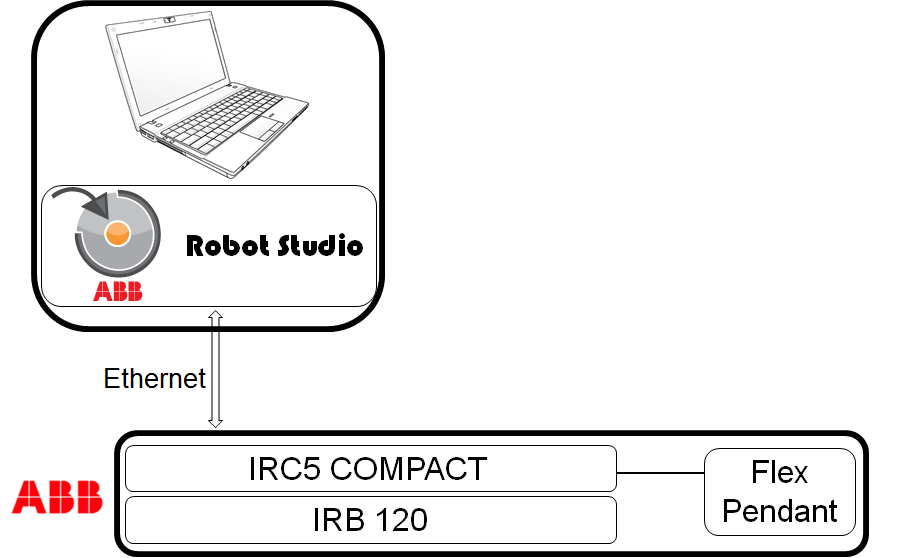
\includegraphics[width=0.75\textwidth]{Immagini/Automatic_SystemSchematic}
	\caption{Schema del funzionamento online del sistema di controllo automatico}
	\label{fig:SchematicAutomatic}
\end{figure}

\chapter{RobotStudio: programmazione statica}
\label{text:RAPID}
Come prima spiegato, \emph{RobotStudio} permette di effettuare una programmazione del movimento che può essere considerata statica: infatti, una volta parametrizzato e settato il codice da fornire al controller IRC5 Compact, non si ha la possiblità di interagire in "tempo reale" con il posizionamento del robot.

Ovviamente la caratteristica "saliente" di una gestione di questo tipo è il fatto che si può operare una pianificazione del movimento in ambito virtuale, sfruttando un controller simulato, il quale offre le stesse funzionalità del controllore fisico, ma solamente riportate su di una piattaforma virtuale.
\begin{figure}[h]
	\centering
	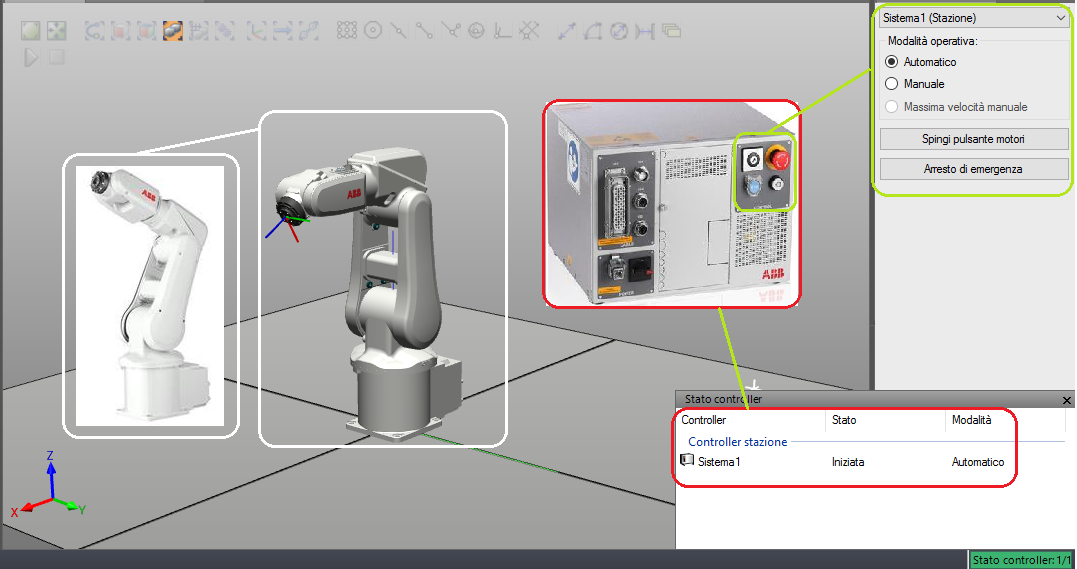
\includegraphics[width=0.85\textwidth]{Immagini/Virtual_System}
	\caption{Virtualizzazione del sistema fisico su piattaforma \emph{RobotStudio}}
	\label{fig:Virtual_sys}
\end{figure}

Nell'ambiente di sviluppo \emph{RobotStudio}, rappresentato nella figura~\vref{fig:Virtual_sys}, si ha un forte orientamento ad una programmazione \emph{statica}: il software mette infatti a disposizione la possibilità di andare a fissare dei sistemi di riferimento (\emph{target}) che, se inseriti all'interno di un percorso (\emph{path}), permettono di definire una movimentazione che il manipolatore poi potrà andare ad eseguire nella realtà, a patto che le posizioni definite dai target siano raggiungibili dal manipolatore stesso, rispettando i limiti e i vincoli geometrici.

La creazione di path è solamente una delle tante possibilità di virtualizzazione che \emph{RobotStudio} mette a disposizione: si possono andare a ricreare sistemi con geometrie molto più complesse come, per esempio, sistemi di saldatura (figura~\vref{fig:Complex_sys}) oppure di pick and place, permettendone così un'analisi del funzionamento e della gestione in maniera completamente svincolata dalla realtà.
Altre funzionalità implementate nell'ambiente di \emph{RobotStudio}, che permettono un controllo più capillare del manipolatore, sono:

\begin{itemize}
	\item Tabelle degli eventi: permettono di verificare la struttura del programma e la sua logica visualizzando gli stati degli I/O.
	\item Rilevamento delle collisioni: si tratta di uno strumento più orientato agli ambienti reali di operazione utilizzato per prevenire possibili collisioni del robot con l'ambiente esterno durante l'esecuzione del programma.
	\item Visual Basic for Applications (\emph{VBA}) per la creazione di interfacce di utilizzo 
\end{itemize}
Tutto questo è però possible, oltre a particolari motori grafici che permettono di modellizzare il sistema reale, anche grazie al linguaggio di programmazione \emph{RAPID}.
\begin{figure}
	\centering
	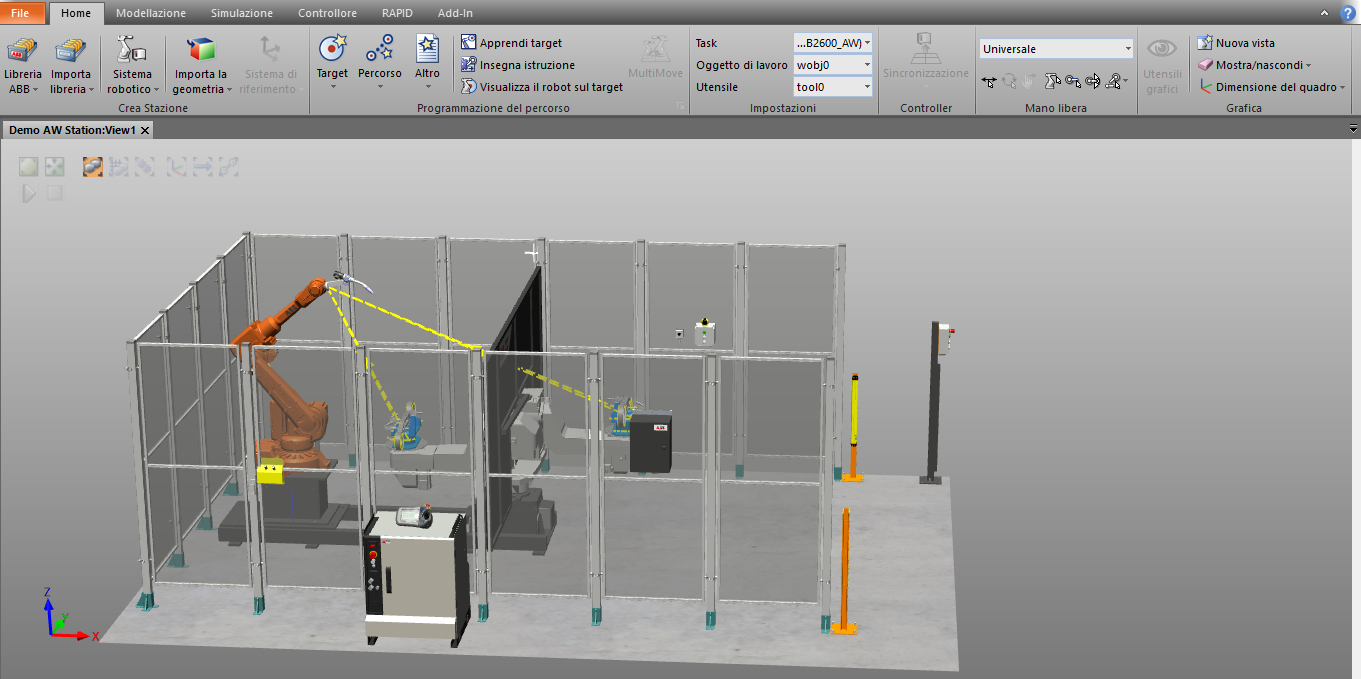
\includegraphics[width=0.8\textwidth]{Immagini/Complex_System}
	\caption{Esemplificazione del livello di complessità dei sistemi simulabili in \emph{RobotStudio}}
	\label{fig:Complex_sys}
\end{figure}

Il cuore della gestione sta quindi nella programmazione: si tratta di un linguaggio ad alto livello steso ad hoc da ABB nel 1994 per poter controllare e gestire la movimentazione dei propri manipolatori, tramite specifiche istruzioni che permettono di definire le modalità, le tempistiche e le velocità di movimento dei robot.
\begin{figure}[h]
	\centering
	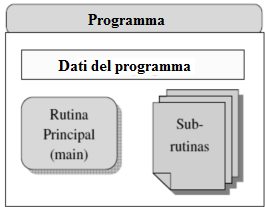
\includegraphics[width=0.45\textwidth]{Immagini/Struttura_RAPID}
	\caption{Schema base della struttura del programma \emph{RAPID}}
	\label{fig:Struttura_RAPID}
\end{figure}

Generalizzando, potremmo dedurre che il programma è una sequenza di istruzioni
che controlla il robot e che generalmente consiste di tre parti (figura~\vref{fig:Struttura_RAPID}): routine principale, subroutine e dati del programma.
\begin{itemize}
	\item Routine principale: routine dove si inizia l'esecuzione (main)
	\item Soubroutine: servono a dividere il programma in parti più piccole	per ottenere un programma modulare
	\item Dati del programma: definire posizioni, valori numerici, sistemi di
	coordinate, ecc. 
\end{itemize}

Quindi, oltre alle più comuni strutture e sintassi di programmazione, sono presenti particolari tipologie di istruzioni (istruzioni per spostare il robot oppure per impostare il valore di un determinato output), il cui comportamento è definito tramite argomenti che gli vengono passati in ingresso, e anche specifiche tipologie di dati, il cui ruolo è mirato ad una più facile gestione del movimento del robot, come si può facilmente notare nel listato~\vref{Code:ExampleRAPID}.

Tutte queste istruzioni che vanno a gestire la movimentazione e la traiettoria del manipolatore ABB possono essere raggruppate in uno o svariati moduli: ciascun modulo può contenere una o svariate procedure.
\label{Text:Mod_sys}
Si possono distinguere:
\begin{description}
	\item[Moduli di programma:] in essi viene memorizzato il codice RAPID che è individuato da un file che con estensione .mod (Module1.mod per esempio).
	Per il controller del robot non fa alcuna differenza se il programma è scritto in più moduli: il motivo di utilizzarne più di uno contemporaneamente in un programma è soltanto quello di rendere più facile la comprensione dello stesso, e agevolandone il riutilizzo da parte dei programmatori. Ovviamente, nonstante sia possibile avere più moduli installati sul controllore, è importante che solamente uno di essi contenga la procedura main, che verrà poi eseguita ripetutivamente dal controller.
	\label{text:SysModule}
	\item[Moduli di sistema:] questa particolare tipologia di moduli, salvati con estensione .sys, permettono di mantenere dati e procedure nel sistema, anche se il programma viene
	cambiato. Ad esempio, se una variabile persistente di tipo \emph{tooldata} viene dichiarata in un modulo di sistema, una calibrazione dell’utensile viene preservata, anche se venisse ad essere caricato un nuovo programma. 
	In questa tipologia di moduli non si ha però la possibilità di inserire delle soubrutine di \emph{main}: ciò significa che l'esecuzione del codice non potrà mai partire da questi moduli, ma dovrà iniziare sicuramente da moduli di programma, i quali poi potranno andare a richiamare le funzioni strutturate all'interno dei moduli di sistema.
\end{description}

\begin{lstlisting}[language=C++,style=Matlab-editor,caption=Esempio di programmazione \emph{RAPID},captionpos=b,label={Code:ExampleRAPID}, basicstyle=\scriptsize\ttfamily,frame=trBL]
MODULE Module1

	CONST robtarget HomePosition:=[[364.302,0,593.9999],[0.498,0,0.802,0],[0,0,0,0],[9E+09,9E+09,9E+09,9E+09,9E+09,9E+09]];
	% NB: La posizione e' definita rispetto al sistema di coordiante oggetto corrente
	CONST robtarget PosizioneIngresso_10:=[[515,325,75],[0,0.604,-0.5,0],[0,0,0,0],[9E+09,9E+09,9E+09,9E+09,9E+09,9E+09]];
	TASK PERS wobjdata Wobj_CellaPiante:=[FALSE,TRUE,"",[[200,200,0],[1,0,0,0]],[[0,0,0],[1,0,0,0]]]; 
	VAR robtarget TargetMobile;
	VAR num NumeroCicli := 0;
	VAR num m := 1;
	CONST robtarget PuntoIntermedio:=[[650,-215.8,150],[0.046,0.007,0.882,-0.002],[0,0,0,0],[9E+09,9E+09,9E+09,9E+09,9E+09,9E+09]];

	PROC main()
		IF (NumeroCicli = 0) THEN
			TPErase;
			%Per limitare le possibilita' di avere singolarita'
			SingArea\LockAxis4;
			MoveL HomePosition,v50,z5,tool0\WObj:=wobj0;
		ENDIF
		IF (NumeroCicli MOD m = 0 AND (NOT(NumeroCicli = 0))) THEN
			Y_Offset := 0;
			X_Offset := X_Offset -21;
		ENDIF
		TPWrite("Offset Y: "+ValToStr(Y_Offset));
		TPWrite("Offset X: "+ValToStr(X_Offset));
		TargetMobileEstrazione := Offs(PartenzaCellaEstrazione,X_Offset,Y_Offset,0);
		TargetMobile := Offs(PartenzaCella,X_Offset,Y_Offset,0);
		Y_Offset := Y_Offset - 22;
		NumeroCicli :=NumeroCicli+1;
	ENDPROC
ENDMODULE
\end{lstlisting}

Presentare però in questa sede il linguaggio \emph{RAPID}, con il giusto livello di approfondimento, sarebbe praticamente impossibile e, al contempo, fuoriluogo: per una maggiore trattazione si rimanda il lettore ai riferimenti \cite{ABB:Manul_RAPID} e \cite{ABB:CompleteManul_RAPID}.

\chapter{Programmazione dinamica: case study}
\label{subsec:ROS}
La pianificazione della traiettoria e la gestione della movimentazione in \emph{RobotStudio} è sicuramente molto "user-friendly": si ha la possibilità di generare automaticamente codice \emph{RAPID} a seconda di come viene configurato il sistema nella sezione di configurazione visuale, creando traiettorie ad hoc, con il minimo sforzo.

Il problema di un approccio di questo tipo è però che non si ha la possibilità di gestire in "tempo-reale" la movimentazione del robot: una volta caricato il listato \emph{RAPID} a bordo del controllore, esso lo eseguirà in maniera ciclica, fino a che non giungerà ad un punto di arresto inserito nel codice oppure fino a quando non verrà arrestato dell'esterno (tramite, per esempio, il fungo d'emergenza).

In progetti molto complessi vi è però spesso la necessità di creare traiettorie adattive, a seconda di quello che è lo stato dell'ambiente in cui il robot si trova a dover lavorare: è necessario quindi sapere gestire la movimentazione del manipolatore a seconda di quelle che sono le informazioni ricevute per esempio da fotocamere, sensori visuali etc. variando in maniera dinamica la posizione e l'orientamento del'end-effector, e quindi del robot stesso, in base al feedback ricevuto.
Nello studio delle diverse possibilità di controllo del manipolatore IRB 120 di ABB sono state prese in considerazioni molte alternative: si è pensato inzialmente di andare a fornire a \emph{RobotStudio} un file con estensione .txt contenente tutte le coordinate che il manipolatore avrebbe dovuto raggiungere. In questa pirma soluzione la parte dinamica sarebbe stata fornita da una scrittura continua del file .txt delle coordinate, in maniera tale che il codice statico struttrato in ambiente \emph{RAPID} potesse poi andare gestire in maniera iterativa la posizione del manipolatore.

Una seconda soluzione presa in considerazione, è stata quella di utilizzare un metodo di controllo basato sulla comunicazione tramite \emph{OPC Server}: OPC (OLE for Process Control) è uno standard di comunicazione nel campo di controllo e supervisione dei processi industriali, basato su una tecnologia Microsoft, che offre un'interfaccia comune per la comunicazione consentendo a singoli componenti software di interagire e condividere dati attraverso un'architettura client-server, il cui ipotetico schema, nel caso di implementazione, sarebbe potuto essere quello in figura~\vref{fig:OPC_Connection}.
\begin{figure}
	\centering
	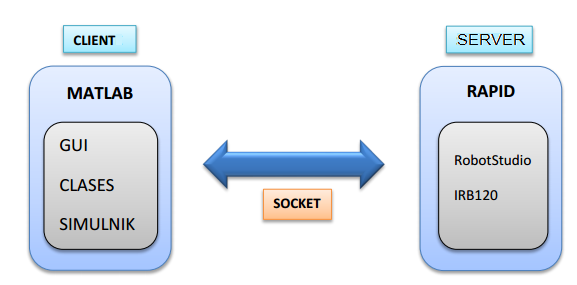
\includegraphics[width=0.75\textwidth]{Immagini/OPC_Configuration}
	\caption{Configurazione di una comunicazione OPC tra client e server}
	\label{fig:OPC_Connection}
\end{figure}

Questo tipo di soluzione è decisamente performante poichè permette di andare a lavorare in ambiente \emph{MATLAB}, tramite alcuni toolbox dedicati che consentono una gestione maggiormente ottimizzata della cinematica inversa, con la possibilità anche di andare a lavorare con sistemi costruiti tramite blocchi in ambiente Simulink.

La terza soluzione, presa poi effettivamente in considerazione, è stata quella di andare ad utilizzare ROS per gestire dinamicamente la traiettoria del manipolatore, a seconda dello stato dell'ambiente: quindi, per la disponibilità di informazioni reperibili sul web, unitamente ad un \emph{know-how} di partenza in ambiente di sviluppo Ubuntu, è stato scelto di andare a seguire e sviluppare un controllo basato su questa opzione.

\chapter{ROS: \emph{Robot Operating System}}
\begin{figure}[h]
	\centering
	
\includegraphics[width=0.3\textwidth]{Immagini/Logo_ROS}
	\caption{\emph{Robot Operating System}}
	\label{fig:LogoROS}
\end{figure}
Andiamo ora ad introdurre, all'interno di questo progetto, una piattaforma software chiamata \emph{Robot Operating System}, più comunemente detta ROS, la quale risulta essere frutto di un enorme sviluppo subito negli ultimi anni dalla comunità della robotica, il quale ha permesso la creazione di algoritmi e ambienti in grado di andare a gestire piattaforme robotiche con un sempre maggiore livello di autonomia e intelligenza.
\begin{figure}[h]
	\centering
	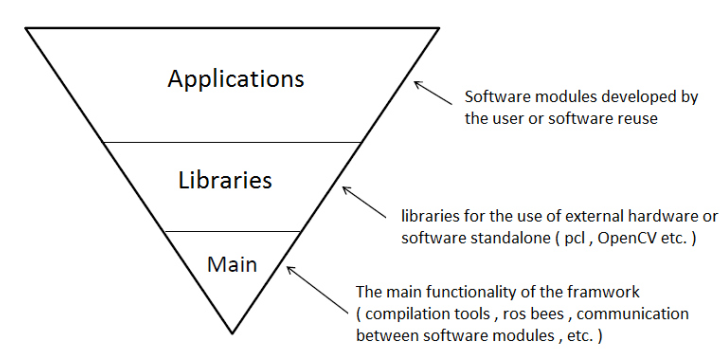
\includegraphics[width=0.75\textwidth]{Immagini/ROS_ComponentBased}
	\caption{Struttura a componenti di ROS}
	\label{fig:ROS-ComponentBased}
\end{figure}

ROS, come si può vedere \cite{online:ROS-Page}, è definibile come:
\begin{center}
	\emph{ROS è un sistema operativo open-source, con una struttura basata su componenti, che fornisce librerie e tools per aiutare gli sviluppatori a creare robot applications. Esso fornisce astrazione dell'hardware, driver dei dispositivi, librerie, strumenti di visualizzazione, comunicazione a scambio di messaggi tra processi (message passing), gestione dei pacchetti e molto altro}.\\	
\end{center}
Prima di entrare nello studio dell'architettura della nostra applicazione, risulta essere utilie andare ad introdurre quelli che sono i componenti principali: ROS, essendo infatti un sistema operativo, crea una rete (figura~\vref{fig:ROS-Network}) dove tutti i processi sono connessi tra di loro. 
\begin{figure}[h]
	\centering
	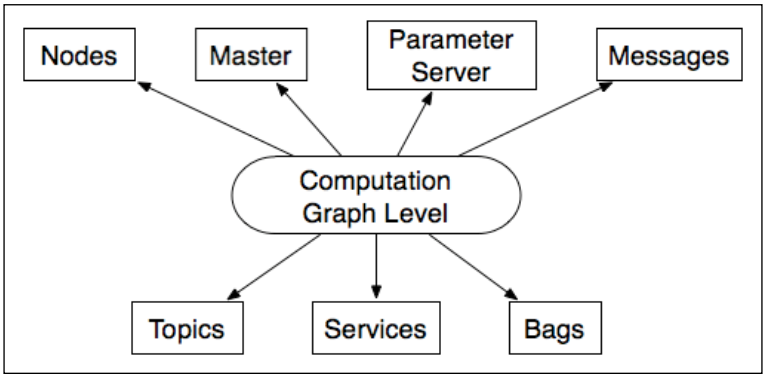
\includegraphics[width=0.75\textwidth]{Immagini/ROS_Network}
	\caption{Concetti fondametali su cui si basa una "network" ROS}
	\label{fig:ROS-Network}
\end{figure}

Nello specifico, all'interno di questa rete, possiamo andare ad individuare diversi elementi caratterizzanti, quali:
\begin{description}
	\item[\underline{Nodes}:] un \emph{nodo} è un processo che esegue delle operazioni di calcolo, fornendo così un modo per poter andare a dividere le funzionalità del sistema in più blocchi, semplificandone di molto il funzionamento e l'utilizzo.
	Le operazioni a cui si fa riferimento sono sostanzialmente implementate tramite l'utilizzo di diverse librerie (ROS client library) come roscpp, che permette di produrre nodi scritti in C++, oppuree rospy, per l'ambiente Python.
	Ogni nodo può andare a comunicare con altri nodi attrraverso \emph{topics}, RPC services oppure tramite \emph{Parameter server}. 
	
	Per comprendere meglio il concetto di nodo, è bene evidenziare come, in un sistema di controllo per sistemi robotici, sono compresi solitamente più nodi, uno per esempio va a controllare gli azionamenti delle ruote, uno ne computa la posizione e un'altro ancora ne calcola il percorso (\emph{path planning}) etc.
	
	Ad ogni singolo nodo è associato un nome univoco all'interno del sistema, in maniera tale che la comunicazione tra di essi possa avvenire senza ambiguità.
	In particolar modo, l'architettura "a nodi" che caratterizza il sistema ROS si basa sul concetto di.
	\begin{itemize}
		\item[Roscore:] il nodo roscore, considerabile come il nodo master, è l'elemento fondamentale che si occupa di andare a coordinare la connessione tra i nodi che sono legati a roscore stesso gestendone la comunicazione.
		\item[Rosnode:] esso rappresenta la tipologia di nodi sviluppati dall'utente, tramite la stesura di codice (solitamente C++ oppure Python).
	\end{itemize}
	\begin{figure}[h]
		\centering
		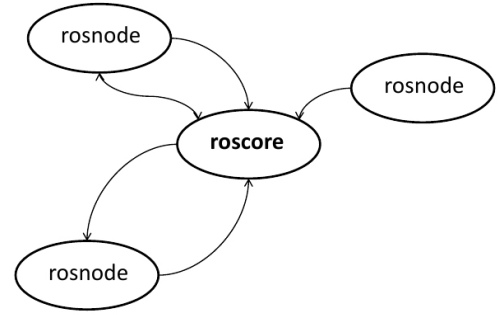
\includegraphics[width=0.75\textwidth]{Immagini/Ros_Core_Node}
		\caption{Elementi principali dell'architettura ROS}
		\label{fig:RosCoreNode}
	\end{figure}

	\item[\underline{Topics}:] essi non sono altro che "bus" attraverso i quali i nodi vanno a scambiarsi messaggi, rendendo possibile una programmazione multi-thread, ignorando i problemi relativi alla sincronizzazione tra processi. Nello specifico, tramite l'utilizzo di topics, si va a creare una semantica "anonima" di comunicazione, definita \emph{publish-subscribers}\label{text:pubsub}, che permette di disaccoppiare, come detto in precedenza, le parti di produzione delle informazione da quelle che le informazioni invece vanno a consumarle.
	
	In questo protocollo di comunicazione e scambio di messaggi, i nodi non sono a conoscenza del destinatario con cui stanno comunicando. Essi sono invece interessati al tipo di dati che si vanno a scambaire tramite un certo topic: infatti, ogni singolo topic, è fortemente tipizzato da ROS, il chè gli consente di avere più subscribers, ma un solo tipo di dato.
	\begin{figure}[h]
		\centering
		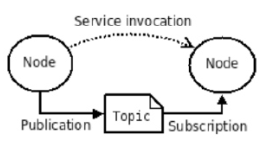
\includegraphics[width=0.70\textwidth]{Immagini/PubSub}
		\caption{Comunicazione basata sul protocollo \emph{publisher-subscribers}}
		\label{fig:PubSub}
	\end{figure}
	
	Questo significa che tramite un dato topic, i nodi che vi sono connessi (\emph{subscribers}), possono scambiarsi solamente una certa tipologia di messaggi: quindi è molto importante sottolineare il fatto che un nodo può diventare \emph{publisher} su un certo topic, solamente se il tipo di messaggio che vuole pubblicare coincide con quello "caratterizzante" il topic in questione e allo stesso tempo può sottoscrivere un topic solamente se la tipologia dei messaggi coincide con quella trattata.
	
	\item[\underline{Services}:] il modello publish/subscriber è sicuramente un paradigma di comunicazione molto flessibile, ma il suo trasporto unidirezionale \emph{molti a molti} non è appropriato per le interazioni di richiesta e risposta tipiche della comunicazione tra nodi. Questo concetto di richiesta/risposta è quindi realizzato tramite \emph{service}, come si vede nella figura \ref{fig:PubSub}, il quale è definito da una coppia di messaggi: uno per la richiesta e uno per la risposta.
	In sostanza un nodo ROS offre un servizio, sotto un certo nome, a tutti gli altri nodi del sistema, i quali possono richiedere il dato servizio iniviando il messaggio di richiesta, attendendone poi la risposta.
	\item[\underline{Messages}:] i nodi comunicano tra di loro pubblicando messaggi all'interno dei topics; nello specifico, questi messaggi sono rappresentati da una semplice struttura di dati, comprendente dei campi tipizzati. Come evidenziato nel punto precedente, i nodi possono anche scambiarsi un messaggio di richiesta e risposta come parte di una chiamata di servizio ROS i quali  sono definiti nei file srv. 
\end{description}
\begin{figure}[h]
	\centering
	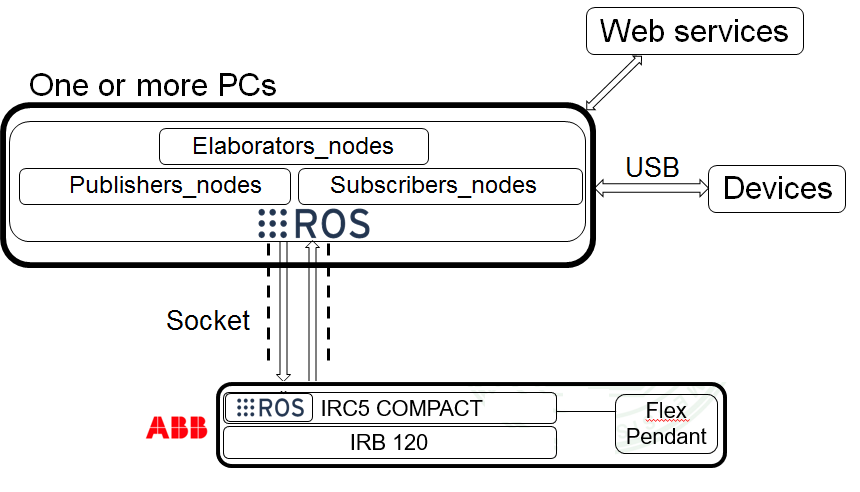
\includegraphics[width=0.75\textwidth]{Immagini/ROS_UniBG_Structure}
	\caption{Struttura architetturale di massima del sistema}
	\label{fig:ROS-UniBG}
\end{figure}
Gli elementi sicuramente caratterizzanti la comunicazione e lo scambio di informazioni all'interno di ROS sono sicuramente i nodi, i quali rappresentano programmi esecutivi che si scambiano dati attraverso topics: ogni singolo topic ha un proprio nome e può accettare solamente un tipo di messaggio.

In ROS sono inclusi molti tipi di messaggi, a seconda della tipologia di informazioni che si ha la necessità di trasmettere: un esempio di messaggio utilizzato molto spesso all'interno di questo progetto è "\emph{geometry\_msgs/Pose}", il quale ha una propria struttura interna composta da 7 variabili di tipo float, 3 delle quali definiscono la posizione e 4 invece rappresentano l'orientamento (espresso in quaternioni).

Per mandare messaggi è quindi necessario eseguire un'azione di \emph{publish} su uno specifico topic per quella data tipologia di messaggi; per riceverli è invece necessario fare un'azione di \emph{subscribe}, ovvero sottoscriversi ad un determinato topic.
\begin{lstlisting}[style=Matlab-editor,caption=Semplice esempio di comunicazione publish-subscribe,captionpos=b,label={Code:pubsub-example}, basicstyle=\scriptsize\ttfamily,frame=trBL]

	%Node 1:
	#include geometry\_msgs/Pose.h
	ros:: Publisher pub = n.advertise<geometry\_msgs::Pose>("object_position",10);
	pub.publish(send\_position);
	
	%Node 2:
	ros::Subscriber sub
	handle_function(geometry\_msgs/Pose received\_position)
	 {
	 	...
	 }
	 ros::Subscriber sub = n.subscribe("object\_position",10,handle_function);
\end{lstlisting}


\section{ROS industrial e IRB 120}
La struttura di ROS presentata in precedenza rappresenta un'architettura generica, la quale però non fornisce gli strumenti adatti per poter andare a gestire la traiettoria e la movimentazione dei manipolatori utilizzati in ambito industriale. Le potenzialità dell'ambiente ROS possono però essere estese anche all'ambito manifatturiero e produttivo, permettendo così di realizzare applicazioni robotiche di produzione che in precedenza erano tecnicamente irrealizzabili e proibitive.

Questo è possibile grazie a \emph{ROS-I} (ROS Industrial) il quale, tramite la presenza di molte repository open source disponibili online, fornisce interfacce per i più diffusi manipolatori industriali, end-effector, sensori e dispositivi connessi in rete, fornendo molti benefici, sostanzialmente dovuti alla forte struttura stratificata che \emph{ROS-I} fornisce (figura~\vref{fig:RosIStructure}).
\begin{itemize}
	\item Aumentare le potenzialità di ROS
	\item Applicare la strada a nuove applicazioni
	\item Rendere la programmazione dei robot più ad alto livello
	\item Ridurre i costi
	\item Essere totalmente open-source con una corposa communità di ricerca e sviluppo 
\end{itemize}

\begin{figure}[h]
	\centering
	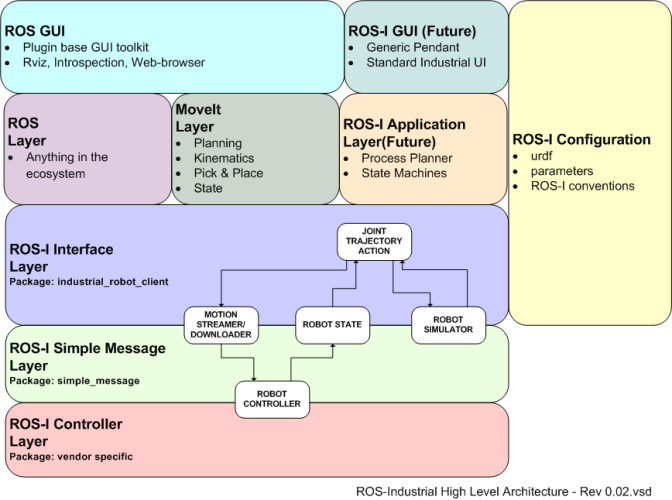
\includegraphics[width=0.75\textwidth]{Immagini/ROS_I_Structure}
	\caption{Architettura ad alto livello di ROS Industrial}
	\label{fig:RosIStructure}
\end{figure}

Volendo quindi andare a gestire la movimentazione di un manipolatore ABB, dovremo essere in grado di dare a \emph{ROS-I} le giuste informazioni in merito alla geometria del robot stesso unitamente alle caratteristiche intrinseche: questo è possibile grazie ai pacchetti software che ROS-Industrial mette a disposizione.
Tali pacchetti possono essere suddivisi in 
\begin{itemize}
	\item Pacchetti software generici, in grado di fornire delle implementazioni non specifiche
	\item Pacchetti software specifici, i quali forniscono supporto per il setup e la configurazione di molte piattaforme robotiche
\end{itemize}
Tra questi pacchetti specifici, troviamo anche quelli che permettono di andare ad eseguire un setup dell'ambiente ROS per quanto riguarda i manipolatori della linea di ABB.
Andiamo quindi ora ad analizzare nello specifico quella che è la struttura \emph{publish-subscriber} che il pacchetto ABB implementato in \emph{ROS-I} mette a disposizione.

\section{Comunicazione socket: concetti base}
Come già precedentemente presentato, il classico flusso di lavoro e di comunicazione tra il robot IRB 120 e il controller IRC5 Compact è schemtizzabile in alcuni semplici passi quali, andare a creare un programma in linguaggio RAPID, simularlo in RobotStudio e caricarlo poi a bordo del controller IRC5 per poterlo eseguirlo.
\begin{figure}[h]
	\centering
	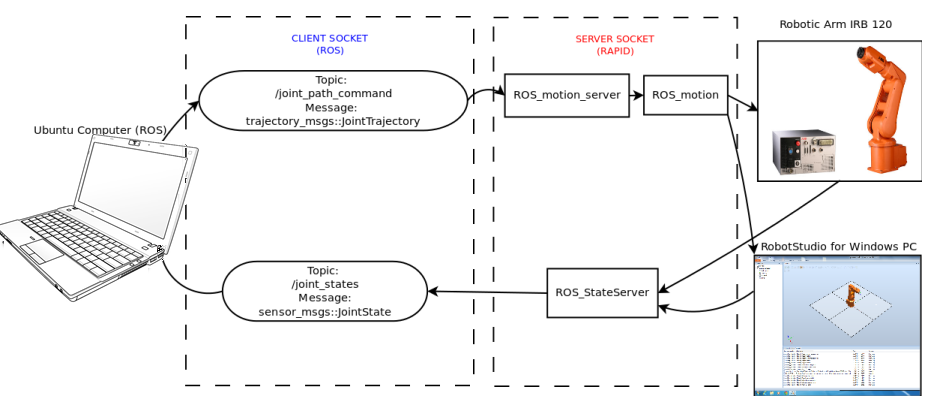
\includegraphics[width=0.75\textwidth]{Immagini/Socket_Comm}
	\caption{Schematizzazione della comunicazione socket tra client e server con relativo flusso di dati}
	\label{fig:SocketStructure}
\end{figure}
Il nostro obbiettivo è quello però di andare ad effettuare un controllo esterno, permettendo l'esecuzione di applicazioni più complesse, come quelle che includono sistemi sensoristici: questa esigenza può essere soddisfatta andando ad utilizzare un socket per permettere al client, ovvero ai nodi in ambiente ROS, di comunicare con il server, che nel nostro caso sarà rappresentato dal controller IRC5 Compact.

Un socket è oggetto software che permette l’invio e la ricezione di dati, tra host remoti (tramite una rete) o tra processi locali (Inter-Process Communication).
Più precisamente, il concetto di socket si basa sul modello Input/Output su file di Unix, quindi sulle operazioni di open, read, write e close; l’utilizzo, infatti, avviene secondo le stesse modalità, aggiungendo i parametri utili alla comunicazione, quali indirizzi, numeri di porta e protocolli.
\begin{figure}[h]
	\centering
	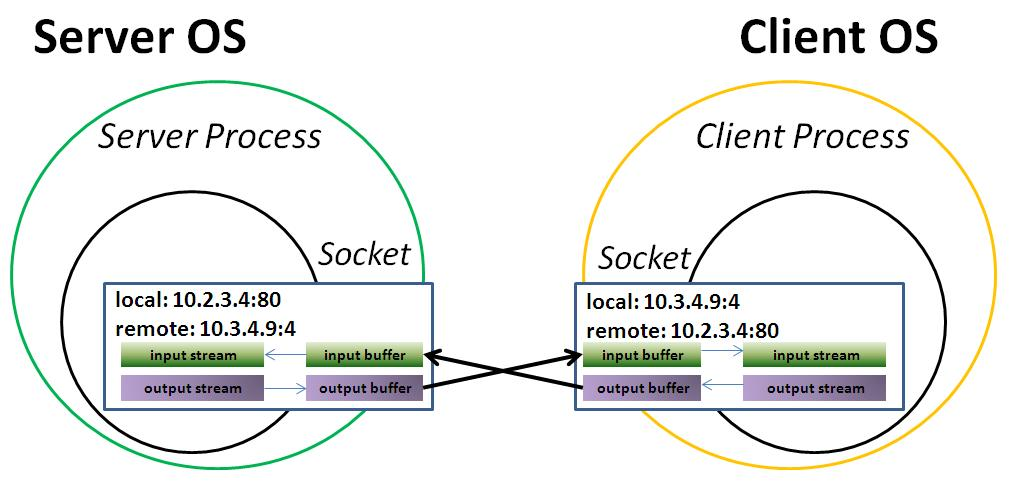
\includegraphics[width=0.75\textwidth]{Immagini/Basic_SocketConfig}
	\caption{Configurazione schematica della comunicazione socket}
	\label{fig:BasicSocketConfig}
\end{figure}

Con tale termine (che letteralmente vuol dire “presa”), in generale, si definisce una rappresentazione a livello software utilizzata per interfacciare due terminali (endpoint) in gioco in una connessione. In altre parole, potremmo considerare i socket come delle prese (una per ogni macchina) che siano interconnesse tra loro attraverso un ipotetico cavo in cui passi il flusso di dati che i computer si scambiano.

Un esempio che rende bene l’idea è quello di pensare ai socket come alle prese telefoniche presenti ai due capi opposti durante una conversazione al telefono. Le due persone che parlano al telefono, comunicano attraverso le rispettive prese. La conversazione, in tal caso, non finirà finché non verrà chiusa la cornetta e fino ad allora la linea resterà occupata.
Questa conversazione deve però essere univocamente individuata dato che, sui sistemi interlocutori, possono esserci molti processi: bisogna quindi avere un modo per indirizzare precisamente il processo con cui si sta dialogando, utilizzando le porte, ovvero numeri che identificano i processi in esecuzione.
Gli interlocutori, quindi, memorizzano indirizzo e porta della controparte, in un indirizzo socket, così formato:
\begin{itemize}
	\item  Indirizzo IP (32 bit)
	\item  Numero di porta (16 bit)
\end{itemize}
In base a come avviene la comunicazione, ovvero lo scambio di pacchetti, si possono avere diverse tipologie di comunicazione socket: in questa applicazione si va a sfruttare la solidità del protocollo TCP (come si può vedere nel listato~\vref{Code:SocketTCP} dove non è specificato l'argomento UDP),
\begin{lstlisting}[style=Matlab-editor,caption=Istruzione RAPID di creazione del socket,captionpos=b,label={Code:SocketTCP}, basicstyle=\tiny\ttfamily,frame=trBL]
IF (SocketGetStatus(server_socket) = SOCKET_CLOSED) SocketCreate server_socket;
\end{lstlisting}
 il quale garantisce una comunicazione affidabile, full-duplex, e con un flusso di byte di lunghezza variabile: essa prende il nome di \emph{Stream socket} e presenta sostanzialmente 4 fasi ben definite, che poi andremo anche a ritrovare nella parte di codice \emph{RAPID}:

\begin{description}
	\item[Creazione del socket:] client e server creano i loro rispettivi socket, e il server lo pone in ascolto su una porta.
	Dato che il server può creare più connessioni con client diversi (ma anche con lo stesso), ha bisogno di una coda per gestire le varie richieste.
	\item[Richiesta di connessione:] il client effettua una richiesta di connessione verso il server.
	Da notare che possiamo avere due numeri di porta diversi, perchè una potrebbe essere dedicata solo al traffico in uscita, l’altra solo in entrata; questo dipende dalla configurazione dell’host.
	In sostanza, non è detto che la porta locale del client coincida con quella remota del server: il server riceve la richiesta e, nel caso in cui sia accettata, viene creata una nuova connessione.
	\item[Comunicazione:] ora client e server comunicano attraverso un canale virtuale, tra il socket del primo, ed uno nuovo del server, creato appositamente per il flusso dei dati di questa connessione.
	È possibile, quindi, che ci siano molti client a comunicare con il server, ciascuno verso il data socket creato dal server per loro.
	\item[Chiusura della connessione:] essendo il TCP un protocollo orientato alla connessione, quando non si ha più la necessità di comunicare, il client lo comunica al server, che ne deistanzia il data socket.
	La connessione viene così chiusa.
\end{description}
\section{Messaggio custom scambiato tramite socket}
\label{text:MessaggeProtocol}
La comunicazione tra client e server, la cui struttura interna sarà spiegata nelle sezioni~\vref{sec:Client} e~\vref{sec:Server}, avviene tramite l'apertura di una connesione socket basata su un protocollo di trasporto di tipo TCP, il quale garantisce una comunicazione più sicura e controllata. Nello specifico client e server si scambiano messaggi che hanno una struttura predefinita, in maniera tale che entrambi siano in grado di interpretare i dati ricevuti/spediti.
Ovviamente questa struttura deve essere definita all'interno dei file di supporto presenti all'interno del \emph{catkin workspace} installato in ambiente Unix: il file che specifica la struttura del messaggio è il file \emph{simple\_message.h} che può essere trovato sotto il percorso \emph{ catkin\_ws\textbackslash src\textbackslash industrial\_core \textbackslash simple\_message\textbackslash include\textbackslash simple\_message.h}.

All'interno di questo file si può vedere come il messaggio sia strutturato in 3 macro-parti:
\begin{description}
	\item[Prefix:] non è considerato parte del messaggio e contiene la lunghezza, in bytes, dell'intero messaggio composto da Header+Body 
	\item[Header:] è formato sostanzialmente da 3 sotto campi i quali rappresentano dei parametri che consentono una corretta identificazione del tipo di messaggio (\emph{message type code}) che si sta mandando e dello stato della comunicazione. Questi campi sono:
	\begin{description}
		\item[MSG\_TYPE: ]permette di identificare il tipo di messaggio tramite dei valori standard e specifici a seconda del tipo di robot con cui si sta lavorando, tramite la dichiarazione di un'enumerazione, come si può vedere nel listato~\vref{Code:MSGTYPE_Param}, il quale è definito sempre all'interno del file \emph{simple\_message.h}.		
		\begin{lstlisting}[style=Matlab-editor,caption=Definizione dei parametri del campo MSG\_TYPE,captionpos=b,label={Code:MSGTYPE_Param}, basicstyle=\tiny\ttfamily,frame=trBL]
			namespace StandardMsgTypes
			{
				enum StandardMsgType
				{
					INVALID = 0,
					PING = 1,
					
					JOINT_POSITION = 10,
					JOINT = 10, 
					READ_INPUT = 20,
					WRITE_OUTPUT = 21,
					
					JOINT_TRAJ_PT = 11,  %Invio dati posizione
					JOINT_TRAJ = 12,	  %Download dei punti della traiettoria
					STATUS = 13,         %Stato in cui si trova il robot
					JOINT_TRAJ_PT_FULL = 14,  %Joint trajectory point message (all message fields)
					JOINT_FEEDBACK = 15,      %Feedback di pos/vel/accel dei joint

					% Definizione del valore inziale dell'enum, a seconda del manipolatore che si sta utilizzando
					
					SWRI_MSG_BEGIN     = 1000,
					UR_MSG_BEGIN       = 1100,
					ADEPT_MSG_BEGIN    = 1200,
					ABB_MSG_BEGIN      = 1300,
					FANUC_MSG_BEGIN    = 1400,
					MOTOMAN_MSG_BEGIN  = 2000
				};
			}
			typedef StandardMsgTypes::StandardMsgType StandardMsgType;
		\end{lstlisting}
		\item[COMM\_TYPE:] codici che permettono di identificare il tipo di comunicazione, indipendentemente dal tipo di robot con cui si sta lavorando. 
		\begin{lstlisting}[style=Matlab-editor,caption=Definizione dei parametri del campo COMM\_TYPE,captionpos=b,label={Code:COMMTYPE_Param}, basicstyle=\tiny\ttfamily,frame=trBL]
			namespace CommTypes
			{
				enum CommType
				{
					INVALID = 0,
					TOPIC = 1,
					SERVICE_REQUEST = 2,
					SERVICE_REPLY = 3
				};
			}
			typedef CommTypes::CommType CommType;
		\end{lstlisting}
		\item[REPLY\_CODE:] dato la presenza di una sistema di feedback che permette di verifcare la corretta movimentazione del manipolatore, è necessario che il server non sia in grado solamente di ricevere traiettorie ma anche di rielaborarle, costruendo un messaggio nel formato standard, e poi inviarle. Si ha quindi la necessità di avere dei parametri che permettono di ritornare informazioni rilevanti in caso di successo oppure di errore.
		\begin{lstlisting}[style=Matlab-editor,caption=Definizione dei parametri del campo REPLY\_CODE,captionpos=b,label={Code:REPLYTYPE_Param}, basicstyle=\tiny\ttfamily,frame=trBL]
			namespace ReplyTypes
			{
				enum ReplyType
				{
					INVALID = 0,
					SUCCESS = 1,
					FAILURE = 2
				};
			}
			typedef ReplyTypes::ReplyType ReplyType;
		\end{lstlisting}
	\end{description}
	\item[Body:] bytearray composto dai dati che effettivamente si vogliono trasferire tra client e server, tra cui anche la posizione che i 6 giunti del manipolatore devono assumere 
\end{description}
Oltre a queste 3 macro-parti in cui è strutturato il messaggio, sono presenti anche dei "\emph{Special sequence code}" i quali permettono di andare a discriminare i vari punti della traiettoria, riconoscendo quelli che sono i punti iniziali e finali della traiettoria stessa, come è descritto nel listato~\vref{Code:Special_Param}.
\begin{lstlisting}[style=Matlab-editor,caption=Definizione dei codici con uso speciale,captionpos=b,label={Code:Special_Param}, basicstyle=\tiny\ttfamily,frame=trBL]
	namespace SpecialSeqValues
	{
		enum SpecialSeqValue
		{
			START_TRAJECTORY_DOWNLOAD  = -1, % Segnale che indica l'inizio della traiettoria
			START_TRAJECTORY_STREAMING = -2, % Inizio effettivo della trasmissione della triettoria
			END_TRAJECTORY  = -3, % Segnale che indica la fine della traiettoria
			STOP_TRAJECTORY = -4  %
		};
	}
	typedef SpecialSeqValues::SpecialSeqValue SpecialSeqValue;
\end{lstlisting}

Quindi, tutti i parametri fin qui definiti all'interno dell'ambiente Unix, devono trovare un'ovvia corrispondenza nel server installato sul controller: questo effettivamente avviene, tramite la definizione di variabili locali, come evidenziato nel codice~\vref{Code:REPLYTYPEParam} caricato a bordo del controller.
\begin{lstlisting}[style=Matlab-editor,caption=Definizione dei parametri del campo REPLY\_CODE,captionpos=b,label={Code:REPLYTYPEParam}, basicstyle=\tiny\ttfamily,frame=trBL]

	CONST num ROS_MSG_TYPE_INVALID       := 0;
	CONST num ROS_MSG_TYPE_JOINT         := 10;  
	CONST num ROS_MSG_TYPE_JOINT_TRAJ_PT := 11;  
	CONST num ROS_COM_TYPE_TOPIC         := 1;
	CONST num ROS_COM_TYPE_SRV_REQ       := 2;
	CONST num ROS_COM_TYPE_SRV_REPLY     := 3;
	CONST num ROS_REPLY_TYPE_INVALID     := 0;
	CONST num ROS_REPLY_TYPE_SUCCESS     := 1;
	CONST num ROS_REPLY_TYPE_FAILURE     := 2;
	
	CONST num ROS_TRAJECTORY_START_DOWNLOAD := -1;
	CONST num ROS_TRAJECTORY_END := -3;
	CONST num ROS_TRAJECTORY_STOP := -4;
	
	CONST num ROS_MSG_MAX_JOINTS := 10;  
\end{lstlisting}

\begin{figure}
	\centering
	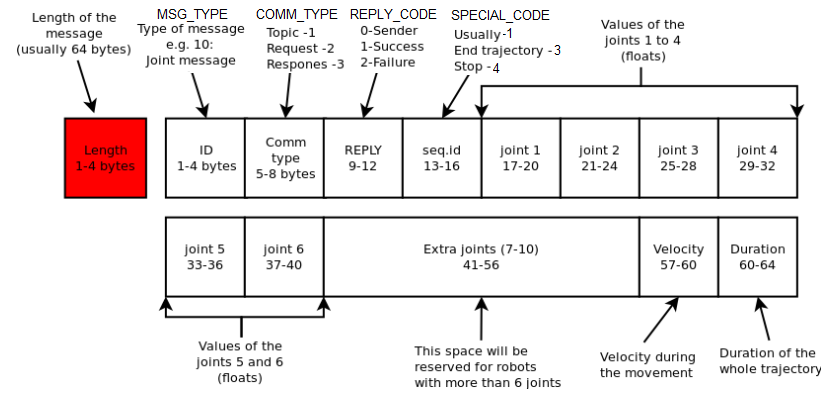
\includegraphics[width=1\textwidth]{Immagini/Message_Protocol}
	\caption{Struttura del messaggio scambiato tra client e server}
	\label{fig:MessageProtocol}
\end{figure}
\section{Client part}
\label{sec:Client}
Nella comunicazione socket che si va ad aprire, siamo in grado di individuare client e server custom per la gestione dei manipolatori ABB.

Le principali funzionalità che un client di questo tipo dovrebbe avere, sono quelle di andare a gestire lo stato corrente dei giunti del manipolatore, ricevendo le informazioni dal controller IRC5 Compact e rielaborandole secondo le necessità.

Il primo step è sicuramente quello di andare ad avviare due packages che si trovano all'interno della nostra applicazione:
\begin{itemize}
	\item abb\_driver
	\item unibg\_robot\_controller
\end{itemize}
Infatti tutto il software ROS, come accennato in precedenza, presenta un'organizzazione a package: nello specifico, un package ROS rappresenta una collezione di file, genericamente sia file eseguibili che di supporto, utilizzati per scopi specifici ed organizzati all'interno di una struttura gerarchica ben precisa (si troveranno sempre due file specifici: il \emph{manifesto} con estensione .xml ed un file \emph{CMakeList}, un file .txt da fornire come input al CMake build per costruire la struttura software dei package).
Nello specifico dei due package sopra riportati, andiamo a lanciare solamente due parti specifiche, che poi andranno ad avviare l'intero insieme dei nodi. Queste parti sono:
\begin{description}
	\item[robot\_interface.launch:] questo file .launch fornisce gli strumenti necessari per andare ad aprire l'effettiva comunicazione socket tra il sistema ROS e il manipolatore ABB, utilizzando il protocollo standard di ROS Industrial spiegato nel paragrafo~\vref{text:MessaggeProtocol}. Possiamo infatti passare a questo particolare tipo di file alcune informazioni chiave, quali l'indirizzo IP del robot da gestire unitamente al file URDF necessario per definire la geometria del manipolatore in uso.
	
	Utilizzando il comando \emph{roslaunch} si è in grado di lanciare files con estensione .launch, permettendo di andare ad avviare più nodi contemporaneamente, quali:
	\begin{description}
		\item[robot\_state:] esso si connette al modulo di programma \emph{State\_Server} caricato a bordo del controller, ed è responsabile della pubblicazione dello stato corrente del robot e del valore in gradi dei 6 giunti del manipolatore. 
		\item[motion\_download\_interface:] gestisce la movimentazione del robot, spedendo al controllore IRC5 Compact punti formanti una traiettoria.
		\item[joint\_trajectory\_action:] si tratta di un nodo che permette di fornire al controller i punti che il manipolatore deve raggiungere (figura~\vref{fig:joint-trajectory-action}) e toccare per seguire una specifica traiettoria, segnalando allo stesso tempo la corretta esecuzione e il raggiungimento dell'obbiettivo.
		
		Questo nodo presenta inoltre la possibilità di imporre dei vincoli alla movimentazione, potendo interrompere l'esecuzione della traiettoria stessa nel momento in cui i vincoli risultano essere violati.  
		\begin{figure}[h]
			\centering
			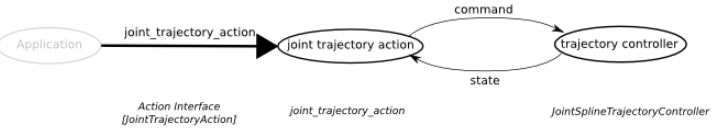
\includegraphics[width=1\textwidth]{Immagini/joint_trajectory_action}
			\caption{Funzionalità del nodo joint\_trajectory\_action}
			\label{fig:joint-trajectory-action}
		\end{figure}
	\end{description} 
	\item[unibg\_simple\_move\_node:] nel punto precedente, l'avvio del file robot\_interface.launch ci ha permesso di avviare contemporaneamente più nodi. In questo caso, utilizzando il comando \emph{rosrun}, andiamo ad avviare un singolo nodo ROS, il quale permette di andare a pubblicare messaggi di tipo \emph{control\_msgs::FollowJointTrajectoryActionGoal} sul topic \emph{joint\_trajectory\_action/goal}.
	
	Nello specifico, il messaggio che viene pubblicato sul topic ha un a struttura ben precisa, la quale è formata da:
	\begin{description}
		\item[std\_msgs/Header header:] esso è utilizzato per trasmettere l'informazione in merito al timestamp della comunicazione unitamente all'identificativo del tipo di sistema di riferimento utilizzato per definire le coordinate (\emph{no\_frame} oppure \emph{global\_frame}).
		\item[actionlib\_msgs/GoalID\ goal\_id:] esso contiene un timestamp che rappresenta l'istante in cui è stata richiesta una certa coordinata; questo istante è utilizzato dal server, posto sul controller, quando tenta di andare ad annullare tutte le traiettorie richieste prima di un certo timeout.
		Oltre al timestamp è presente un campo identificativo univoco che permette di associare un certo feedback ad una specifica traiettoria.
		\item[control\_msgs/FollowJointTrajectoryGoal\ goal:] in questo campo del messaggio pubblicato dal nostro nodo unibg\_simple\_move\_node si vanno a definire tra parametri importanti:
		\begin{description}
			\item \emph{goal\_time\_tolerance}: indica la tollerenza temporale entro il quale si impone il raggiungimento del punto stabilito
			\item \emph{path\_tolerance e goal\_tolerance}: se la misura dei parametri di joint di velocità, poisizione e accelerazione cade fuori dal range di tolleranza, la traiettoria è abortita.
			\item \emph{trajectory\_msgs/JointTrajectory trajectory}: qui è contenuta l'informazione più importante, ovvero quella che riguarda i punti che vanno a comporre la traiettoria, unitamente al nome dei joint.
		\end{description}		
	\end{description}
	L'informazione contenuta nel messaggio denominato precedentemente come \emph{goal} sarà quindi poi pubblicato dal nostro nodo, tramite i comandi mostrati nel listato~\vref{Code:TopicsPub}.
	\begin{lstlisting}[style=Matlab-editor,caption=Pubblicazione messagio \emph{trajectory} di esempio nel topic corrispondente,captionpos=b,label={Code:TopicsPub}, basicstyle=\tiny\ttfamily,frame=trBL]
		ros::Publisher pub_joint_action = n.advertise<control_msgs::FollowJointTrajectoryActionGoal>("joint_trajectory_action/goal", 1);
		control_msgs::FollowJointTrajectoryActionGoal goal;

		goal.goal.trajectory.header.stamp = ros::Time::now() + ros::Duration(1.0);
		int ind = 0;
		goal.goal.trajectory.points[ind].positions.resize(6);
		goal.goal.trajectory.points[ind].positions[0] = -1.3963;
		goal.goal.trajectory.points[ind].positions[1] = 0.65;
		goal.goal.trajectory.points[ind].positions[2] = 0.5461;
		goal.goal.trajectory.points[ind].positions[3] = 0.0;
		goal.goal.trajectory.points[ind].positions[4] = 0.3747;
		goal.goal.trajectory.points[ind].positions[5] = 0.0;
		goal.goal.trajectory.points[ind].time_from_start = ros::Duration(5.0);
	\end{lstlisting}
\end{description}
Gli elementi caratterizzanti il sistema sono però i topic: infatti, una volta avviati i nodi (per mezzo dei comandi \emph{rosrun} e \emph{roslaunch}), nascono alcuni topic specifici, i quali possono andare a scambiare solamente determinate tipologie di messaggi (per la struttura dei messaggi legati ai singoli topic fare riferimento a \cite{online:ROS-api}). I topic che si creano, come si può vedere nella figura~\vref{fig:rosgraph} sono:
\begin{itemize}
	\item /feedback\_states
	\item /joint\_path\_command
	\item /joint\_trajectory\_action/cancel
	\item /joint\_trajectory\_action/feedback
	\item /joint\_trajectory\_action/goal
	\item /joint\_trajectory\_action/result
	\item /joint\_trajectory\_action/status
	\item  /robot\_status
\end{itemize}
\begin{figure}
	\centering
	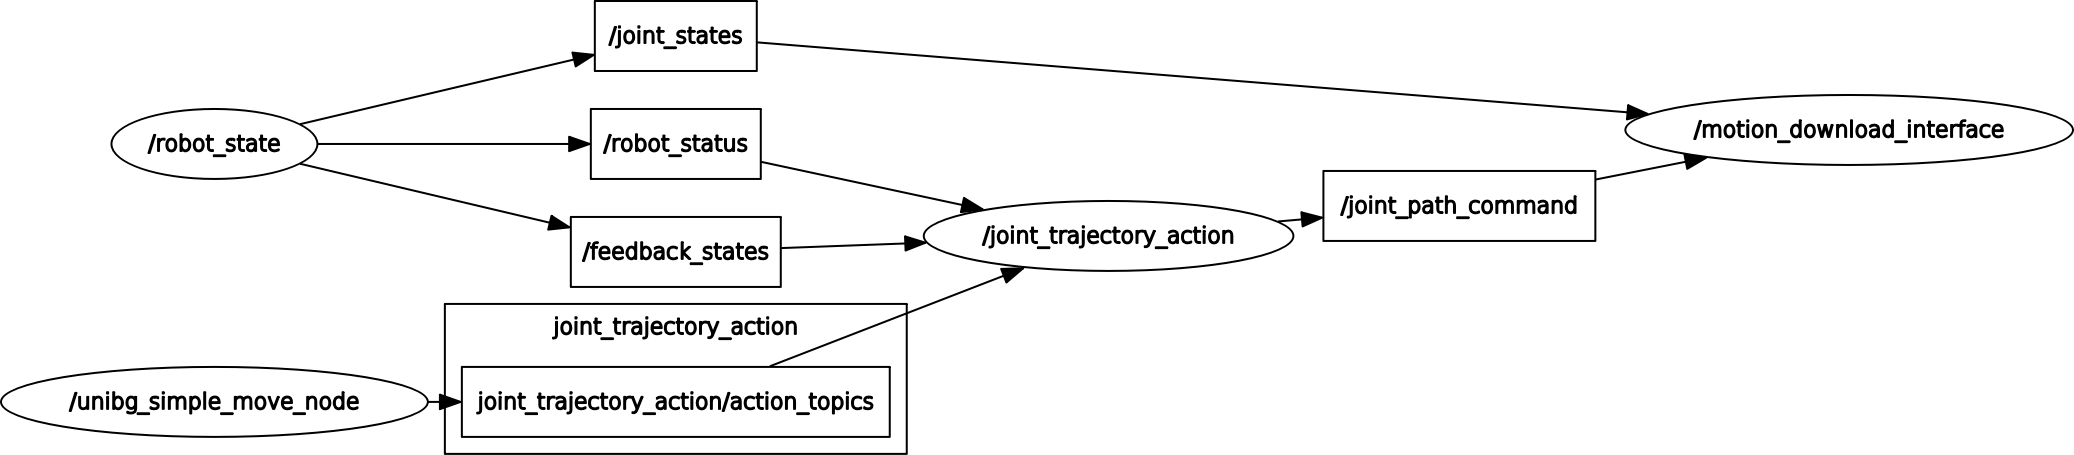
\includegraphics[width=1.3\textwidth]{Immagini/rosgraph}
	\caption{Grafo delle dipendenze tra topics e nodi}
	\label{fig:rosgraph}
\end{figure}
\section{Architettura ABB ROS Server}
Come visto in precedenza (capitolo~\vref{text:pubsub}), il fulcro del controllo tramite ROS sta proprio in un continuo scambio di messaggi sul modello \emph{publisher-subscriber}: essa può essere quindi considerata come una struttura client-server, dove il client è rappresentato da un insieme di nodi \emph{ROS} in grado di pubblicare particolari tipologie di messaggi (sezione~\vref{sec:Client}). 

Il server è invece rappresentato, per forza di cose, dal controllore IRC5 Compact, il quale deve essere in grado di andare a ricevere le informazioni necessarie per gestire la traiettoria del robot, per mezzo dell'instaurazione di una comunicazione tramite socket.

Per poter andare a configurare il controllore è necessario fare riferimento ancora all'ambito di programmazione \emph{RobotStudio}: in questo caso però, una volta configurato il codice RAPID e caricato a bordo del controller stesso, non avremo più bisogno di modificare la struttura, poichè la traiettoria verrà gestita direttamente dall'ambiente ROS, ottenendo il comportamento dinamico desiderato.
Nello specifico risultano essere necessari tre task: 
\begin{itemize}
	\item T\_ROB1
	\item ROS\_StateServer
	\item ROS\_MotionServer
\end{itemize}
\begin{figure}
	\centering
	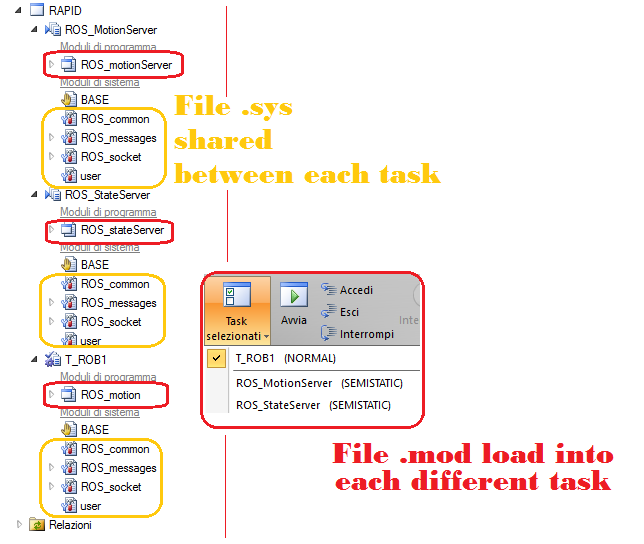
\includegraphics[width=0.75\textwidth]{Immagini/ParallelTask_VirtualController}
	\caption{Struttura multitasking del server ROS implementato in codice RAPID}
	\label{fig:ParallelTask}
\end{figure}

La struttura principale della nostra applicazione \emph{RAPID} è quindi formata da più task, i quali procedono la loro esecuzione in parallelo, a partire dal momento in cui l'esecuzione inzia, fino ad un tempo potenzialmente infinito(a meno di errori presenti all'interno del codice stesso): non tutti e tre i task hanno però lo stesso peso e le stesse funzionalità, come si può vedere nella figura~\vref{fig:TaskConfiguration}. 
\label{text:TROB1}

Il task T\_ROB1 rappresenta l'unico task che può andare gestire direttamente la movimentazione del manipolatore tramite istruzioni di movimento, essendo configurato come \emph{Motion Task}: per le proprietà della programmazione in RobotStudio, qualsiasi task impostato come task di movimento, deve essere di tipo NORMAL, ovvero deve poter essere eseguito in primo piano. Questo implica che, per andare a movimentare il manipolatore, è necessario, come primo step, andare ad attivare questo task.

ROS\_StateServer e ROS\_MotionServer sono invece configurati come task SEMISTATIC: si tratta quindi di task in \emph{background}, il cui funzionamento non può essere controllato, ovvero vengono eseguiti automaticamente nel momento in cui il controllore viene avviato.
\begin{figure}[h]
	\centering
	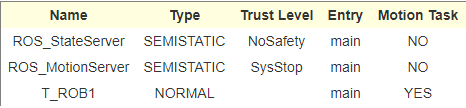
\includegraphics[width=0.75\textwidth]{Immagini/Task_Configuration}
	\caption{Configurazioni dei task del ROSserver}
	\label{fig:TaskConfiguration}
\end{figure}

Questa rappresenta però la struttura "statica" dei task che vanno a comporre il server ROS (sezione~\vref{sec:Server}): in ognuno di esso è necessario andare a caricare moduli di programma contenenti le istruzioni RAPID da eseguire. Si tratta dei moduli \emph{ROS StateServer.mod, ROS MotionServer.mod e TROB\_1}, ai quali vanno aggiunti anche i moduli di sistema \emph{ROS common.sys, ROS socket.sys e ROS messages.sys}, i quali risultano essere condivisi tra tutti i task. 

La parte "dinamica" dell'intera applicazione risulta essere invece sviluppata e costrutita in ambiente Unix, grazie alle funzionalità offerte dal sistema operativo ROS (sezione~\vref{sec:Client}).




\section{Server part}
\label{sec:Server}
\subsection{ROS\_MotionServer}
Essendo che il modulo caricato all'interno del task omonimo si trova in continua esecuzione, una volta che viene stabilita la connessione socket tra client e server, esso inizia a ricevere messaggi contenenti i punti formanti le traiettorie inviate dal client ROS, come si può vedere nel listato:
\begin{lstlisting}[style=Matlab-editor,caption=Ricezione delle traiettorie con relativo controllo d'integrità,captionpos=b,label={Code:ROSMotionServer},basicstyle=\scriptsize\ttfamily,frame=trBL]
	LOCAL CONST num server_port := 11000;
	
	LOCAL VAR socketdev server_socket;
	LOCAL VAR socketdev client_socket;
	LOCAL VAR ROS_joint_trajectory_pt trajectory{MAX_TRAJ_LENGTH};
	LOCAL VAR num trajectory_size;
	
	PROC main()
		VAR ROS_msg_joint_traj_pt message;
		
		TPWrite "MotionServer: Waiting for connection.";
		ROS_init_socket server_socket, server_port;
		ROS_wait_for_client server_socket, client_socket;
		
		WHILE ( true ) DO
			ROS_receive_msg_joint_traj_pt client_socket, message;
			trajectory_pt_callback message;
		ENDWHILE
		
	ERROR (ERR_SOCK_TIMEOUT, ERR_SOCK_CLOSED)
		IF (ERRNO=ERR_SOCK_TIMEOUT) OR (ERRNO=ERR_SOCK_CLOSED) THEN
			SkipWarn;  
			ErrWrite \W, "ROS MotionServer disconnect", "Connection lost.  Resetting socket.";
			ExitCycle;  % restart program
		ELSE
			TRYNEXT;
		ENDIF
	UNDO
		IF (SocketGetStatus(client_socket) <> SOCKET_CLOSED) SocketClose client_socket;
		IF (SocketGetStatus(server_socket) <> SOCKET_CLOSED) SocketClose server_socket;
	ENDPROC
\end{lstlisting}

Nella ricezione dei punti che compongono una data traiettoria è però importante andare a distinguerne due: il punto iniziale e il punto finale.

Quindi, unitamente alla ricezione del messaggio per mezzo della procedura ROS\_receive\_msg\_joint\_traj\_pt condivisa tramite il modulo di sistema ROS\_messages, si va a richiamare la procedura locale trajectory\_pt\_callback la quale, con una semplice struttura switch case effettuata sul campo \emph{sequence\_id} del messaggio, permette di andare a verificare che tipo di punto stiamo andando ad analizzare.
\begin{lstlisting}[style=Matlab-editor,caption=Struttura che permette di riconoscere la natura del punto da aggiungere alla traiettoria in esame,captionpos=b,label={Code:ROSMotionServer2},basicstyle=\scriptsize\ttfamily,frame=trBL]
	TEST message.sequence_id
		CASE ROS_TRAJECTORY_START_DOWNLOAD:
			TPWrite "Traj START received";
			trajectory_size := 0;                 % Reset  della trajectory size
			add_traj_pt point;              
		CASE ROS_TRAJECTORY_END:
			TPWrite "Traj END received";
			add_traj_pt point;                    
			activate_trajectory;
		CASE ROS_TRAJECTORY_STOP:
			TPWrite "Traj STOP received";
			trajectory_size := 0;  %
			activate_trajectory;
			StopMove; ClearPath; StartMove; 
		DEFAULT:
			add_traj_pt point;            
	ENDTEST
\end{lstlisting}


\subsection{ROS\_StateServer}
Il compito principale del modulo di programma contenuto in questo task, è quello di andare ad inviare messaggi broadcast contenenti informazioni e dati in merito alla posizione dei giunti.
In particolar modo la funzionalità di questo modulo, il quale rimane in esecuzione continuamente in background, è molto importante: esso permette, una volta stabilita la connessione socket, di inviare al client, ad un determinato rate (\emph{update\_rate}), la posizione corrente dei 6 giunti. 

Si chiude così l'anello di retroazione, tramite un feedback che risulta essere molto importante per quelle applicazioni in cui è necessaria un'elevata precisione nella movimentazione.  
\begin{lstlisting}[style=Matlab-editor,caption=Feedback continuo della posizione del manipolatore,captionpos=b,label={Code:ContinuosFeedBack},basicstyle=\scriptsize\ttfamily,frame=trBL]
	LOCAL CONST num server_port := 11002;
	LOCAL CONST num update_rate := 0.10;  % broadcast rate (sec)
	
	LOCAL VAR socketdev server_socket;
	LOCAL VAR socketdev client_socket;
	
	PROC main()
	
		TPWrite "StateServer: Waiting for connection.";
		ROS_init_socket server_socket, server_port;
		ROS_wait_for_client server_socket, client_socket;
		
		% Spedizione con periodo pari a update_rate del valore attuale dei joint
		WHILE (TRUE) DO
		send_joints;
		WaitTime update_rate;
		ENDWHILE
\end{lstlisting}

\subsection{ROS\_Motion: effettiva movimentazione del manipolatore}
In questo task, all'interno del modulo caricatovi a bordo, come anticipato nel paragrafo~\vref{text:TROB1}, avremo le effettive istruzioni che vanno a mettere in movimento il robot, essendo che esso è caricato all'interno del task T\_ROB1, il quale è definito come l'unico \emph{Motion Task}. 

Il concetto base è che dall'ambiente ROS, più nello specifico dal modulo ROS\_motion\_server.mod, si ricevono un insieme di punti (o \emph{targets}), i quali vanno a comporre la traiettoria che il manipolatore dovrà andare a seguire.

In sostanza si scandisce con un ciclo tutta la lista dei target, la cui lettura è eseguita nella soubrutine \emph{init trajectory()}, tramite l'utilizzo di un lock sulla lettura cosicchè nessuno vada sovrascrivere la traiettoria mentre se ne sta effettuando l'acquisizione.
\begin{lstlisting}[style=Matlab-editor,caption=Movimentazione effettiva del manipolatore,captionpos=b,label={Code:ROSMotion}, basicstyle=\scriptsize\ttfamily,frame=trBL]

	% Il server e' settato per ricevere una serie di target e poi andare ad eseguire un insieme conosciuto di posizioni, non dando la possibilita' di aggiungere target "on-the-fly"
	
	LOCAL VAR ROS_joint_trajectory_pt trajectory{MAX_TRAJ_LENGTH};
	LOCAL VAR num trajectory_size := 0;
	LOCAL VAR intnum intr_new_trajectory;
	
	PROC main()
		VAR num current_index;
		VAR jointtarget target;
		VAR speeddata move_speed := v10;  % velocita' di default
		VAR zonedata stop_mode;
		VAR bool skip_move;
				
		WHILE true DO
			% La variabile "ROS_new_trajectory" e' una variabile di tipo "PERSistent bool", la quale permette di mantenere l'ultimo valore salvato, anche in caso di interruzione dell'esecuzione, ed e' necessaria per segnalare se e' disponibile o meno una nuova traiettoria
			IF (ROS_new_trajectory)
				% Acquisizione, con lock, della traiettoria
				init_trajectory;
			
			% Analizzo i punti componenti la traiettoria
			IF (trajectory_size > 0) THEN
				FOR current_index FROM 1 TO trajectory_size DO
					%Acquisisco i valori in gradi dei 6 giunti
					target.robax := trajectory{current_index}.joint_pos;
					
					% Se il primo punto e' vicino (entro i limiti di tolleranza) al punto da raggiungere, allora devo saltare questo target
					skip_move := (current_index = 1) AND is_near(target.robax, 0.1);
					IF (current_index = trajectory_size) 
						stop_mode := fine;  % stop at path end
					
					%=====================================================
					% Effettiva esecuzione del movimento
					IF (NOT skip_move)
						MoveAbsJ target, move_speed, \T:=trajectory{current_index}.duration, stop_mode, tool0;
					%=====================================================
				ENDFOR
				
				trajectory_size := 0;  % movimentazione eseguita
			ENDIF
			
			WaitTime 0.05; 
		ENDWHILE
		
		ERROR
			ErrWrite \W, "Motion Error", "Error executing motion.  Aborting trajectory.";
			abort_trajectory;
	ENDPROC
\end{lstlisting}

\subsection{ROS\_Socket: apertura della connessione socket lato server}
Nell'archietettura del server, ROS\_socket rappresenta un modulo di sistema (vedi~\vref{text:SysModule}): esso quindi risulta essere condiviso tra tutti i task, i quali hanno quindi la possibilità di richiamare le funzioni che vi sono al suo interno. 
Nello specifico, il modulo di sistema in esame, contiene 4 routine che permettono di gestire l'interazione con il socket, le quali sono:
\begin{description}
	\item[ROS\_init\_socket:] in questa funzione si vanno a definire i parametri della connessione, quali l'indirizzo IP e il numero della porta, e successivamente la si va a creare, associandolo alla variabile di tipo \emph{socketdev} fornita in ingresso alla funzione.
	\begin{lstlisting}[style=Matlab-editor,caption=Analisi funzionamento routine ROS-init-socket ,captionpos=b,label={Code:ROSinitsocket}, basicstyle=\scriptsize\ttfamily,frame=trBL]
		% SocketGetStatus e' un istruzione che restituisce lo stato corrente di un socket, il quale puo' essere:
		 - SOCKET_CREATED
		 - SOCKET_CONNECTED
		 - SOCKET_BOUND
		 - SOCKET_LISTENING
		 - SOCKET_CLOSED
		% Se non esiste alcuna connessione socket la vado a creare 
		IF (SocketGetStatus(server_socket) = SOCKET_CLOSED) SocketCreate server_socket;
		
		% Se il socket e' stato gia' creato allora associo al socket stesso l'indirizzo ip specificato del server e il numero della  sua porta. Da evidenziare il fatto che l'indirizzo del server e' ottenuto automaticamente, come indirizzo del controller tramite l'istruzione GetSysInfo
		
		IF (SocketGetStatus(server_socket) = SOCKET_CREATED) SocketBind server_socket, GetSysInfo(\LanIp), port;
		
		% Qui il controller, che lavora come un server, inizia effettivamente ad ascoltare e ricevere le comunicazioni in ingresso
		IF (SocketGetStatus(server_socket) = SOCKET_BOUND) SocketListen server_socket;
	\end{lstlisting}
\end{description}
\begin{description}
	\item[ROS\_wait\_for\_client:] con questa funzione si va a stabilire l'effettiva connessione tra client e server della comunicazione socket.
	
	Nello specifico in questa funzione, si ha una gestione della connessione che possiamo definire "temporizzata": infatti, tra i parametri di input è presente la variabile numerica facoltativa \emph{wait\_time} che permette di specificare la quantità massima di tempo riservata all'esecuzione del programma per l'attesa di connessioni in arrivo. Nel caso in cui questo tempo scada, senza che giunga alcuna connessione in ingresso, si andrà a generare un errore (ERR\_SOCK\_TIMEOUT) che poi verrà ad essere gestito.
	\begin{lstlisting}[style=Matlab-editor,caption=Analisi funzionamento routine ROS-wait-for-client,captionpos=b,label={Code:ROSwaitforclient}, basicstyle=\scriptsize\ttfamily,frame=trBL]	
		VAR string client_ip;
		VAR num time_val := WAIT_MAX; 		

		% Essendo il parametro wait\_time facoltativo, devo verificare che sia presente
		IF Present(wait_time) time_val := wait_time;
		
		IF (SocketGetStatus(client_socket) <> SOCKET_CLOSED) SocketClose client_socket;
		WaitUntil (SocketGetStatus(client_socket) = SOCKET_CLOSED);
		
		% L'istruzione SocketAccept, utilizzabile solamente lato server, permette di andare ad accettare una connessione in arrivo: una volta accettata la connessione, lo stato del socket diventa di SOCKET_LISTENING
		
		SocketAccept server_socket, client_socket, \ClientAddress:=client_ip, \Time:=time_val;
		TPWrite "Client at "+client_ip+" connected.";
	\end{lstlisting}
\end{description}
\begin{description}
	\item[ROS\_receive\_msg:] questo routine è prevalentemente utilizzata dal modulo di sistema \emph{ROS\_messages.sys}, il quale se ne serve per andare a salvare momentaneamente in una variabile "buffer" i dati ricevuti dalla comunicazione socket, tramite l'utilizzo dell'istruzione \emph{UnpackRawBytes}, necessaria per raggruppare il contenuto di un contenitore di tipo rawbytes.
	
	Successivamente tutti i dati ricevuti vengono inseriti all'interno della variabile message, che è quindi pronta per la conversione e per essere elaborata.
	\item[ROS\_send\_msg:] questa routine riceve la posizione corrente dei joint del manipolatore, all'interno di una variabile di tipo \emph{ROS\_msg}. I dati, in formato raw bytes, sono analizzati, riuniti secondo la struttura del messaggio del protocollo (sezione~\vref{text:MessaggeProtocol}) ed infine vengono spediti attraverso il socket. 

	Si tratta quindi di una comunicazione di feedback del server verso il client: in sostanza permette al codice sviluppato in ROS di verificare la correttezza della movimentazione.
\end{description}
\subsection{ROS\_messages}
In questo modulo di sistema, si vanno a creare 4 tipologie di variabili utilizzate per contenere i dati inerenti alle traiettorie e ai punti che le compongono. Sono presenti inoltre 2 procedure che permettono di operare una trasformazione e uno scambio di messaggi.
\begin{description}
	\item[ROS\_receive\_msg\_joint\_traj\_pt:] in questa procedura si va a convertire il messaggio \emph{raw\_message}, mandato dal client, nella variabile \emph{message}.
	Si tratta di variabili che hanno sostanzialmente una struttura diversa: \emph{raw\_message} è una variabile di tipo ROS\_msg la cui struttura è riporta nel listato seguente, mentre \emph{message} è la variabile che viene effettivamente utilizzata per effettuare la movimentazione desiderata, ed essa è di tipo ROS\_msg\_joint\_traj\_pt, la cui struttura è invece riportata nel listato~\vref{Code:RecordROSmsgjointtrajpt} e nella figura~\vref{fig:MessageProtocol}.
	\begin{lstlisting}[style=Matlab-editor,caption=Campi caratterizzanti il tipo di variabili ROS-msg,captionpos=b,label={Code:RecordROSmsg}, basicstyle=\scriptsize\ttfamily,frame=trBL]	
		RECORD ROS_msg
			num msg_type;
			num comm_type;
			num reply_code;
			rawbytes data;
		ENDRECORD
	\end{lstlisting}
	\begin{lstlisting}[style=Matlab-editor,caption=Campi caratterizzanti il tipo di variabili ROS-msg-joint-traj-pt,captionpos=b,label={Code:RecordROSmsgjointtrajpt}, basicstyle=\scriptsize\ttfamily,frame=trBL]	
		RECORD ROS_msg_joint_traj_pt
			num msg_type;
			num comm_type;
			num reply_code;
			num sequence_id;
			robjoint joints;  % in gradi
			num velocity;
			num duration;
		ENDRECORD
	\end{lstlisting}
	
	Il trasferimento effettivo da una forma di messaggio all'altra, che altro non è che il cuore di questa procedura, unitamente alla conversione in gradi, è riportato nel codice~\vref{Code:Unpack}.
	\begin{lstlisting}[style=Matlab-editor,caption=Unpacking del messaggio ricevuto dal client,captionpos=b,label={Code:Unpack}, basicstyle=\tiny\ttfamily,frame=trBL]	
		UnpackRawBytes raw_message.data, 1, message.sequence_id, \IntX:=DINT;
		UnpackRawBytes raw_message.data, 5, message.joints.rax_1, \Float4;
		UnpackRawBytes raw_message.data, 9, message.joints.rax_2, \Float4;
		UnpackRawBytes raw_message.data, 13, message.joints.rax_3, \Float4;
		UnpackRawBytes raw_message.data, 17, message.joints.rax_4, \Float4;
		UnpackRawBytes raw_message.data, 21, message.joints.rax_5, \Float4;
		UnpackRawBytes raw_message.data, 25, message.joints.rax_6, \Float4;
		% Skip bytes 29-44.  UNUSED.  Reserved for Joints 7-10.
		UnpackRawBytes raw_message.data, 29+(ROS_MSG_MAX_JOINTS-6)*4, message.velocity, \Float4;
		UnpackRawBytes raw_message.data, 33+(ROS_MSG_MAX_JOINTS-6)*4, message.duration, \Float4;
		% Convert data from ROS units to ABB units
		message.joints := rad2deg_robjoint(message.joints);
	\end{lstlisting}
	\item[ROS\_send\_msg\_joint\_data:] in questa routine invece si va ad effettuare un'operazione nella direzione opposto di quella compiuta all'interno della procedura ROS\_receive\_msg\_joint\_traj\_pt. Si ricostruiscee quindi la struttura del messaggio adatta per essere inviata al client, come feedback.   
	\begin{lstlisting}[style=Matlab-editor,caption=Packing del messaggio per spedizione verso il client come mezzo di feedback,captionpos=b,label={Code:Pack}, basicstyle=\tiny\ttfamily,frame=trBL]	
		PackRawBytes message.sequence_id, raw_message.data,  1, \IntX:=DINT;
		PackRawBytes ROS_joints.rax_1,    raw_message.data,  5, \Float4;
		PackRawBytes ROS_joints.rax_2,    raw_message.data,  9, \Float4;
		PackRawBytes ROS_joints.rax_3,    raw_message.data, 13, \Float4;
		PackRawBytes ROS_joints.rax_4,    raw_message.data, 17, \Float4;
		PackRawBytes ROS_joints.rax_5,    raw_message.data, 21, \Float4;
		PackRawBytes ROS_joints.rax_6,    raw_message.data, 25, \Float4;
		FOR i FROM 1 TO ROS_MSG_MAX_JOINTS-6 DO   % Insert placeholders for joints 7-10 (message expects 10 joints)
		PackRawBytes 0,               raw_message.data, 25+i*4, \Float4;
		ENDFOR
		
		ROS_send_msg client_socket, raw_message;
	\end{lstlisting}
\end{description}
%=================================================================================